\documentclass[conference]{IEEEtran}
% generated by Docutils <http://docutils.sourceforge.net/>
\usepackage{fixltx2e} % LaTeX patches, \textsubscript
\usepackage{cmap} % fix search and cut-and-paste in Acrobat
\usepackage{ifthen}
\usepackage[T1]{fontenc}
\usepackage[utf8]{inputenc}
\usepackage{float} % float configuration
\floatplacement{figure}{H} % place figures here definitely
\usepackage{graphicx}

%%% Custom LaTeX preamble
% PDF Standard Fonts
\usepackage{mathptmx} % Times
\usepackage[scaled=.90]{helvet}
\usepackage{courier}
\usepackage{graphicx}
\usepackage{amsmath}
\usepackage{tabularx}
\usepackage{multirow}
\usepackage{flushend}
\usepackage{url}
\bibliographystyle{IEEEtran}

%%% Title Data
\title{Comparative API Complexity Analysis of Two Platforms for Networked Multiplayer Games using a Reference Game}
\author{
  \IEEEauthorblockN{
    Toni Alatalo\IEEEauthorrefmark{1}\IEEEauthorrefmark{2}\IEEEauthorrefmark{3},
    Erno Kuusela\IEEEauthorrefmark{1}\IEEEauthorrefmark{2}\IEEEauthorrefmark{3},
    Rauli Puuperä\IEEEauthorrefmark{1}\IEEEauthorrefmark{3},
    and Timo Ojala\IEEEauthorrefmark{1}
  }
  \IEEEauthorblockA{\IEEEauthorrefmark{1}Department of Computer Science and Engineering, University of Oulu, Finland}
  \IEEEauthorblockA{\IEEEauthorrefmark{2}Center for Internet Excellence, University of Oulu, Finland}
  \IEEEauthorblockA{\IEEEauthorrefmark{3}Playsign Ltd., Oulu, Finland}
}

\begin{document}
\maketitle
\begin{abstract}
In this paper we propose the quantitative analysis of the complexity
of a simple reference game implemented on a particular gaming platform
as means for characterizing how the platform succeeds in easing the
development of networked multiplayer games. We first present our own
open source tool based on Sneed’s Object-Point (OP) method for the
automatic quantitative assessment of the complexity of a software API
by analyzing a source code using the API. We then apply our tool,
together with the recently released JSComplexity tool based on
classical software complexity metrics, to compare two platforms for
networked multiplayer games, the open source realXtend Tundra SDK and
the proprietary Union. As the reference games we use existing
implementations of the simple Pong game atop the two platforms. Our
data shows that these complexity metrics reveal API design tradeoffs,
resulting in complexity differences in the reference games.
\end{abstract}

\section{Introduction}
Reusable software libraries and platforms are pivotal for managing
complexity in game development. Their APIs virtualize underlying
functionality, including but not limited to: game entity management,
scene construction, mathematics, input events, rendering graphics, gui
input widgets, asset retrieval, game data networking, user
authentication and data storage. Thus, APIs are essential for
productive game development. It has been noted how making good APIs is
hard - and that creating a bad API is easy \cite{api-matters}. Even a
small quirk in an API can accumulate to substantial problems in larger
bodies of application source code. API design has a significant impact
on software quality, and increased API complexity is associated with
increased software failure rates \cite{cmu-api_failures}.

Also single player games encompass rich multifaceted functionality,
but networked multiplayer games are typically much more complex. In
network programming the developer needs to deal with events, conflicts
and error conditions originating from other parts of the distributed
system as well as the local user. This is emphasized in multiuser
real-time systems when compared to the relatively leisurely
request-response interaction patterns of most client-server
applications. Developing a massively multiplayer online game (MMOG)
has been estimated to typically take two to three times longer than
creating and launching a single-player game \cite{middleware}.

Rigorous quantitative assessment of a gaming platform in terms of ease
and productivity of development is very challenging. Hsiao and Yuan
\cite{middleware} proposed four essential ``ease of'' requirements for
a MMOG middleware: ease of development, deployment, maintenance and
change. However, they noted the difficulty of quantitatively measuring
the ease of development or change, and focused only on platform
scalability in their evaluation.

We propose to use the implementations of reference game(s) as means
for comparing the “ease of” dimension of game APIs. In this article we
examine how the quantitative analysis of a reference game implemented
atop a particular game development platform enables us to characterize
how the platform succeeds in reducing development complexity. Thus, we
need two things: a method for quantitative analysis of software
complexity, and reference game(s). The collection of reference games
effectively mimics a common corpus that for example in the information
retrieval research is often used to compare the performance of
different information retrieval algorithms.

Inspired by recent progress in quantitative techniques for software
complexity analysis \cite{cmu-api_failures,api-complexity-analysis},
we first propose a tool based on Sneed’s Object-Point (OP) method for
the quantitative assessment of the complexity of a software API based
on the automatic analysis of a source code using the API. Then we use
the tool to compare Tundra’s API complexity to that of the Union
platform with pre-existing implementations of the Pong game on the two
platforms, i.e. Pong serves as the minimal reference implementation of
a networked multiplayer game in our study. As a complementary API
complexity analysis method we use the recently introduced JSComplexity
tool based on classical software complexity metrics
\cite{jscomplexity}. Our study shows that the API complexity metrics
calculated from the reference games with the tools indeed successfully
quantify the different amounts of complexity that the game developer
has to manage on these two alternate platforms.

Our underlying motivation is understanding how the API of the open
source realXtend Tundra SDK, recently introduced by Alatalo
\cite{Alatalo2011}, succeeds in hiding the complexity of networked
multiplayer games. We plan to use the insight and the complexity
measures in on-going development of the platform and an even
friendlier API.

This paper is organized as follows. After briefly reviewing related
work on API complexity analysis we present our tool. Then we report
our case study on using the tool to compare the API complexity of the
two platforms in the development of the Pong game. We conclude the
paper with a discussion on various aspects of the study.

\section{Related Work on API Complexity Analysis}

A wide range of qualitative and quantitative approaches have been
proposed for assessing the complexity of software APIs. The API
usability research has adapted traditional qualitative usability
evaluation methods of the HCI field such as thinking aloud, heuristic
evaluation and cognitive walkthroughs into evaluating APIs
\cite{overview}. Employed metrics include the completion times of
predefined tasks, for example.

In comparison to task-based usability evaluation of GUIs, API
evaluation based on human observations is challenging. When developing
a small application can take even weeks, fitting valid evaluation tasks
into an observation session lasting typically 1-2 hours is difficult
\cite{conceptmaps}. The recently introduced peer review
\cite{apipeerreview} and the concept maps \cite{conceptmaps} methods
address this problem by involving real world usage of an API over a
long period of time. However, they are still considerably laborious
and yield only qualitative findings.

Recently, statistical (quantitative) methods have been proposed for
analyzing the complexity of software APIs. Cataldo and de Sousa
\cite{cmu-api_failures} studied two large corporate software projects
and nine open source projects and found a link between the API
complexity and the failure proneness of the software quantified by the
number of bug reports from the field. They quantified the complexity of
an API by simply calculating the number of public methods and
attributes. The approach is subject to severe limitations as it fails
to take into account pre- and post-invocation assumptions and possible
invocation sequences.

de Souza and Bentolila \cite{automatic-api-eval} introduced the Metrix
tool that evaluates an API by calculating Bandi’s software metrics for
interface size, interaction level and operation argument complexity
from the API specification. After analysing eleven different APIs with
the Metrix tool, de Souza and Bentolila concluded that calculating
such simple metrics directly from the API specification can produce
misleading results. A more complete API may appear more complex, even
if it provides good abstractions that allow completing a particular
task at hand with only a small subset of the API.

An alternative to evaluating the complexity of an API with simple
metrics calculated from the API specification is to assess the
complexity of programs developed using the API. Sobernig et
al. \cite{api-complexity-analysis} proposed exactly this in their
comparative study of the complexity of four different API designs. To
characterize the complexity of a particular API, they applied Sneed’s
\cite{Sneed} Object-Point (OP) analysis to software realized atop the
API. The key is to apply a surrogate measurement so that a program
developed using an API is analyzed, not the API specification itself.

Osmani\cite{todomvc} published TodoMVC, a collection of “To Do” web
application implementations built with various Javascript web
frameworks. Here the source codes of the minimal implementations are
meant for people to read for comparative evaluations. We propose the
same approach for networked games but combined with automated
quantitative analysis.

\section{API Complexity Analysis Tools}

A tool facilitating automated and quantitative analysis of the
complexity of an API from an existing body of source code developed
using the API would provide several advantages. First, real world
data, i.e. source codes of existing applications, could be
utilized. Second, in comparison to manual methods, the analysis would
be faster with immediate feedback and would require much smaller
amount of human labor. Third, longitudinal studies of API development
would be straightforward to conduct by analyzing successive software
versions. A fully automated analysis could be embedded into the
continuous integration of a software bundle, to characterize the
evolution of its complexity over time.

\subsection{Our Tool Based on Sneed’s Object-Point (OP) Method}

Following the work of Sobernig et al. \cite{api-complexity-analysis},
we base our tool on Sneed’s Object-Point (OP) method \cite{Sneed}.
However, in contrast to their manual data collection, our tool
automatically extracts the data needed by the OP method from a
program’s source code. The OP method uses intermediate UML models as
the data to compare programs in different languages. Importantly, the
OP method allows direct tracking between indicator values and program
structures, which is elementary in evaluating API designs. For
example, if many codebases get a high proportion of their complexity
value due to a specific part of an API, it can then be examined
qualitatively.

So called API hotspots and coldspots have been previously
automatically mined from source code \cite{spotweb}. There, however,
the specific parts of an API are not analyzed as sources of complexity,
but simply to identify how much they are used. Their source code
mining is similar to our tool that also needs to identify which
functions are called and how often to employ the OP method.

\subsubsection{Sneed's Object-Point (OP) Method}

Although the OP method was originally developed for deriving early
work estimates from UML design diagrams, recently it has also been
applied to analyzing the complexity and cost of existing software
implementations. While the early COCOMO software cost models used
simply program size (LOC, lines of code) to estimate development
effort, later the more versatile Function-Point, the Data-Point and
finally the Object-Point methods have emerged to incorporate
functionality and other program properties into the cost estimate
\cite{henrich97repositorybased}.

Sobernig \emph{et al.} illustrated the relative robustness of the OP
method to the simple LoC metric on two software implementations. The
first software had only 48 LoC but resulted in 356.34 OP. The second
software had 144 LoC but only 266.76 OP. Their reasoning was: “an API
user is only exposed to an API feature chunk of low structural
complexity”, as “the chunks size is limited in terms of participating
classes and the smallest number of operations per class” and it “shows
a relatively weak connectedness of classes, resulting from the small
number of associations and generalizations between the classes”
\cite{api-complexity-analysis}. This reasoning is of utmost relevance
to our objective of easing the development of networked game
development with good API designs in Tundra. We pursue a limited set
of powerful abstractions with clear interactions that a game developer
could easily learn and grow to master. Not all source code lines are
equal - a poorly designed API makes it a struggle to get even a few
operations working if the developer has to strive for functionality
scattered around in an incoherent way.

The Object-Points, as applied here, are a sum of two parts: Class
Points (CP) and Message Points (MP).

\textbf{Class Points (CP)} (Eq. 1-4) are calculated from the static class structure: the
class count and sums of attribute, operation and relation
counts. Weights are employed to correct the values for the overall
calculation. Class inheritance is taken into account by calculating
novelty weights for specializing classes.

\textbf{Message Points (MP)} (Eq. 5-8) are defined by the set of operations
(functions/methods) \emph{actually used} in the software. First, the number
of operations is recorded. Then, the parameter count for each called
operation is collected. Also, the source and target counts of the
operation calls are established. Again, novelty weights are used to
compensate for repeated occurrences due to subclassing.

\small
\begin{align}
CP &= \left(W_C |C| + \sum_{c_ \in C} |A_c| + W_{R_C} \sum_{c \in C} |R_c| + W_{O_C} \sum_{c \in C} |O_c| \right) \overline{N_C},\\ &\text{where}\\
\overline{N_C} &= \frac{\sum_{c \in C} N_c}{|C|},\, \text{and}\\
N_c &=
\begin{cases}
1,& \text{if class is novel}\\
0.5,& \text{if class has a super class}\\
\end{cases}
\end{align}
\begin{align}
MP &= \left(W_{O_M} |O_M| + \sum_{o \in O_M} |P_o| + W_{S_O} \sum_{o \in O_M} |S_o| + W_{T_O} \sum_{o \in O_M} |T_o| \right) \overline{N_{O_M}},\\ &\text{where}\\
\overline{N_{O_M}} &= \frac{\sum_{o \in O_M} N_o}{|O_M|},\,\text{and}\\
N_o &=
\begin{cases}
1,& \text{if operation is novel}\\
0.5,& \text{if operation is provided by super class}\\
\end{cases}
\end{align}

\begin{tabularx}{\linewidth}{rX}
\hline
$C, |C|...$ & Set of classes, Class count \\
$|A_c|...$  & Attribute count per class   \\
$|O_c|...$  & Operation count --''--      \\
$|R_c|...$  & Relation count --''--       \\
$N_c...$    & Novelty weight of class c \\
$\overline{N_C}$ & Avg. class novelty \\
$|O_M...$  & Set of called operations \\
$|O_M|...$ & Called operation counts \\
$|P_o|...$ & Parameter count of operation o \\
$|S_o|...$ & Source count --''-- \\
$|T_o|...$ & Target count --''-- \\
$N_o...$   & Novelty weight --''-- \\
\end{tabularx}
\normalsize

The weights are adopted directly from the earlier usage of OP for API
complexity analysis, which further uses the standard Data Points
analysis values by Sneed \cite{Sneed}.

\subsubsection{Extracting Object-Point Data from Source Code}

To obtain the static class data for the Class Points (CP), we utilize
existing source code parsing and annotation systems in the API
documentation tools. The first alternative implementations for a
minimal networked game on different modern high-level APIs studied
here are written as a Javascript application and a combination of
Actionscript (as3) for the client and Java for the server module. We
have developed parsers for the internal intermediate representations
of class and method signatures in JsDoc JSON and AsDoc XML
formats. The class information is read by a Python application to an
internal model which contains the data for the OP calculation,
implemented in another module in the same Python application.

To calculate the Message Points reflecting the dynamic function calls,
we use the Closure Javascript compiler to traverse the source code to
collect function calls and their argument counts. A parser made with
Python is used to read the function call data required to calculate
the MPs.

While our tool calculates complete Class Point data, it currently
omits two factors in Message Point data: the source and target counts
of the interactions, and the novelty weight. While the tool tallies
separate calls to each called function in the source code, it is not
yet clear how to map them into the MP values. Sobernig et al. always
set the source and target counts to 1. For the novelty weight we
should check for each called operation called whether it is
implemented in that class or inherited from a superclass. Our tool
does not currently know the class of the object in which an operation
is called. These omissions are not expected to affect the OP values
significantly, at least not to the extent undermining the conclusions
of this study.  

Finally, to facilitate manual validation and visual communication of
the data extracted from the source codes, our tool also creates UML
class diagrams from the very same in-memory data structure that is
used in the OP calculation. We chose the UXF format of the open source
Umlet GUI diagram tool, due to its simple and straightforward XML
format and the even simpler plaintext syntax used to describe
individual UML elements, such as a class or a relation. This allows
further manual editing of the diagrams with the GUI tool to improve
the layout and annotation with notes. We are not aware of any previous
implementation of directly extracting data for the OP method from the
source code. Repository based automatic queries for OP analysis have
been presented earlier by Henrich
\cite{henrich97repositorybased}. There, a repository of documents, or
abstract software design models (PCTE), was queried using the P-OQL
language.

\subsection{JSComplexity}

JSComplexity is a recently released tool for analyzing the software
complexity of JavaScript projects \cite{jscomplexity}. It reports four
different types of complexity metrics of which we use the cyclomatic
complexity and the maintainability index.  Cyclomatic complexity
introduced by McCabe \cite{mccabe} counts the number of linearly
independent paths through a source code. Lower values are better and
McCabe suggested using ten as a threshold value, beyond which modules
should be split into smaller units.  The maintainability index
introduced by Oman et al. \cite{oman} is calculated as follows: 171 -
(3.42 * ln(mean effort)) - (0.23 * ln(mean cyclomatic complexity)) -
(16.2 * ln(mean logical LOC)).

The maintainability index gets values on a logarithmic scale ranging
from negative infinity up to 171, with larger values indicating a
higher level of maintainability. Oman et al. identified 65 as the
threshold value below which a program should be considered difficult
to maintain.

\section{Case Setup}

\subsection{Pong as a Reference Game}

We propose using the Pong game as a minimal networked multiplayer
reference game in the subsequent API complexity analysis. While Pong
is tiny in its functionality, it is still sufficient for demonstrating
key challenges in networked games, given the functional combination of
the clients controlling their own paddles and the ball bouncing in the
shared space. Pong has been used in networked game research earlier,
recently in an interesting study of latency compensation techniques
\cite{pong-ping}. Also, even a minimal game such as Pong reveals the
amount of software needed for the basic functionality: launching the
networked game, establishing connections, handling players joining in
and dropping out, and synchronizing gaming events.

\subsection{Game Platforms}

We briefly introduce the two game platforms whose API complexity we are
going to compare, the open source realXtend Tundra SDK
\cite{Alatalo2011} and the Union, a proprietary closed source
product\footnotemark[1]. Both are relatively high-level platforms for
networked games and bear several interesting similarities and
differences for this study. Both are specifically designed for
networking, which is exposed to the developer at an abstract
application level. That is, the developer and the game do not have to
know anything about sockets or network hosts. Instead, an abstract
container object is provided (Room in Union, Scene in Tundra) and the
game application logic listens to events from the container, for
example when a new client joins the shared session/space. Also, both
platforms provide an automated mechanism for synchronizing shared
state over network. The shared state is stored in special attributes
(objects of type Attribute) residing in the container (in Union
directly in the Room object, in Tundra in the Components of the
Entities in a Scene). The attributes are automatically shared among
all participants, and notifications are provided for parties that have
subscribed to be notified of changes. This way it is simple to for
example set the game scores on the server, and show it in the client
GUIs.

\footnotetext[1]{\url{http://www.unionplatform.com/}}

However, the two platforms also have fundamental differences and we
discuss how they manifest in the implementation of the Pong
game. TundraPong\footnotemark[2] was implemented by the leading author
of this paper and an independent developer in two sessions totaling
about six hours. UnionPong\footnotemark[3] was downloaded from the
Union website, where it is available as a tutorial example. While
TundraPong is a script running atop the Tundra platform, UnionPong is
a client application, to which networking functionality has been added
by using Union’s Reaktor Flash library. TundraPong utilizes a complete
static scene datafile, where the game logic moves objects around. It
runs on an existing client-server system, and utilizes several default
components of the platform, most notably the data defining visual
appearance and spatial instantiation and movement. In contrast,
UnionPong not only has code to create the appearance of the game court
(as it is called in Court.as), but also to define the data required for
the spatial movement of an object (PongObject has x, y, direction,
speed, width and height). In TundraPong, the predefined built-in
Placeable component contains the position and the Rigidbody component
contains shape information for collisions and speed vector for
movement.

\footnotetext[2]{\url{https://github.com/realXtend/doc/tree/master/api_complexity/PongMultiplayer}}
\footnotetext[3]{\url{http://www.unionplatform.com/?page_id=1229}}

Thus, it is clear from the outset that UnionPong is more complex, due
to the game code containing a much larger proportion of the
implementation of the functionality. The upcoming API complexity
analysis is still useful as it helps to answer the questions at hand:
a) how the two APIs succeed in hiding the complexity from the
developer and b) how our tool succeeds in evaluating the relative
complexity of the two APIs.

\subsection{API Complexity Data}

The complexity metrics of the two Pong implementations is presented in
Table 1. We first discuss the OP values provided by our tool. As
anticipated, TundraPong has clearly smaller OP values. For TundraPong
the OP data is extracted from the single Javascript source file
(assets/game.js) that contains both client and server functionality in
two respective classes, with GUI and minimal game session
management. UnionPong has separate client and server source code files
in different languages using different libraries. Therefore, to
facilitate more equal comparison, for TundraPong we also provide the
OP data for the client only, even though it is included in the same
source code file.

For UnionPong the OP data is calculated for all 14 client side
ActionScript files and for selected 8 classes related to networking
(GameManager, GameStates, KeyboardController, PongClient, PongObject,
RoomAttributes, RoomMessages, UnionPong). The excluded classes cover
GUI, the 2D scene implementation and general settings and utilities
(clamp, ClientAttributes, Court, HUD, Rectangle and
Settings). KeyboardController is included because it sends remote
control messages from the player to the server (modifies
client.paddle’s attributes and says client.commit()).

UnionPong’s Java server component (PongRoomModule.java) contains two
classes: PongRoomModule (implements Module, Runnable) and PongObject,
which is basically a duplicate of the same class in the client. As our
OP data extraction tool does not yet support Java, we collected the OP
data from the server component manually.

Overall, the OP values appear useful for characterizing the overall
complexity. The values seem to reflect the functionality that the
application needs to cover with its own code, versus the ready-made
functionality provided by the platform --- complete scene geometry,
physics and basic client-server functionality in Tundra.

\begin{table}[!t]
%% increase table row spacing, adjust to taste
\renewcommand{\arraystretch}{1.3}
% if using array.sty, it might be a good idea to tweak the value of
% \extrarowheight as needed to properly center the text within the cells
\caption{Complexity metrics for the two Pong Implementations}
\label{table_example}
\centering
%% Some packages, such as MDW tools, offer better commands for making tables
%% than the plain LaTeX2e tabular which is used here.
\begin{tabular}{|c|c|c|c|c|c|}
\hline
\multirow{2}{*}{metric} & \multicolumn{2}{c|}{Tundra Pong} & \multicolumn{3}{c|}{Union Pong} \tabularnewline
\cline{2-6}
& Full & Client & Client Full & Client Net & Server \tabularnewline
\hline
LoC     & 361 & 115 & 565 & 420 & 281 \\
\hline
$|C|$   & 2   & 1   & 14  & 8   & 2   \\
CP      & 75  & 27  & 180 & 140 & 75  \\
MP      & 103 & 63  & 196 & 175 & 87  \\
OP      & 178 & 90  & 376 & 315 & 162 \\
\hline
\sum{Cyclom.} & 35  & 16  & 58  & 49  & -  \\
max Cyclom.   & 11  & 11  & 11  & 11  & 13 \\ 
Maint.Idx.    & 100 & 105 & 119 & 116 & -  \\
\hline
\end{tabular}
\end{table}

Regarding the values from the JSComplexity tool, the cyclomatic
complexity is fine-grained, scoring points for individual
functions. It is relevant as the actual programming work is eventually
done in functions, whereas class structures and such are only
containers for code, after all. The aggregate cyclomatic complexity
value is not very useful as it is simply a sum of the values of
individual functions. That is, even the simplest functions with the
minimal complexity value of 1 increase the sum, thus the aggregate
value tells more about the size of the codebase than its
complexity. The aggregate cyclomatic complexity values correlate with
Sneed’s class points (CP) as they involve also operation count. The
real usefulness of the cyclomatic complexity is in identifying peak
values, i.e. individual functions with high complexity. Interestingly,
the maximum cyclomatic complexity value of 11 occurs in a similar
functions in both reference implementations: TundraPong’s
GameServer.updateGame, GameClient.onServerData and UnionPong’s
GameManager.updateBall. These functions implementing the basic logic
of ball movement and bouncing are indeed quite similar. This alludes
that the complexity of the actual game mechanics is quite equal in
both implementations. This in turn suggests that the two platforms do
not differ much with respect to the complexity of basic mechanics such
as moving objects despite the software implementations being quite
different. The same maximum cyclomatic complexity value of 11 in the
TundraPong client side function onServerData is just a coincidence:
the complexity is due to the game session handling commands being made
with JSON and handled in if blocks in a single function. But again,
the equivalent updateBall function implementing ball movement,
bouncing and boundary checks in the UnionPong server has the highest
cyclomatic complexity value of 13.

Finally regarding the maintainability indices it is worthwhile to note
how the values are better for the otherwise larger and more complex
Union Pong implementation. This is due to the different programming
styles of the reference implementations. TundraPong has a smaller
number of larger functions yielding a higher maintainability index. In
contrast, UnionPong has many minimal classes and small functions
resulting in a low index. TundraPong’s maintainability index of 100 is
still well above the 65 threshold proposed by Oman et al. In any case,
these partly contradicting complexity values highlight how the
reference implementations should be as comparable as possible in terms
of structure and programming style, to leave the API as the only
potential source for the complexity. We propose such carefully crafted
reference implementations to be made in future work.

\subsection{UML Diagrams%
  \label{uml-diagrams}%
}

Figures 1 and 2 show the UML diagrams generated from the OP data by
our tool for subsequent manual verification of the analysis and the
API complexity.
\begin{figure}
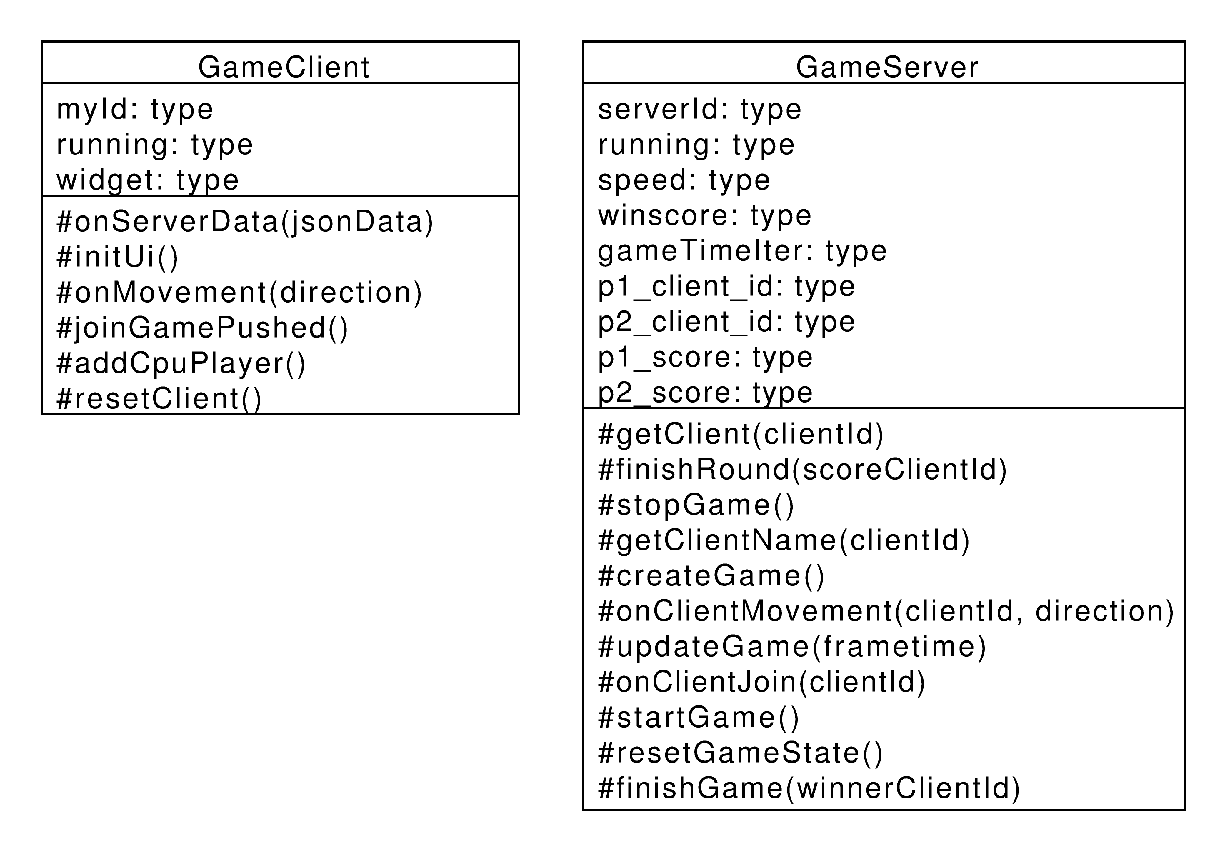
\includegraphics[scale=0.400000]{pics/TundraPong_fontembed.pdf}
\caption{The two classes in TundraPong game.js.}
\end{figure}
\begin{figure}
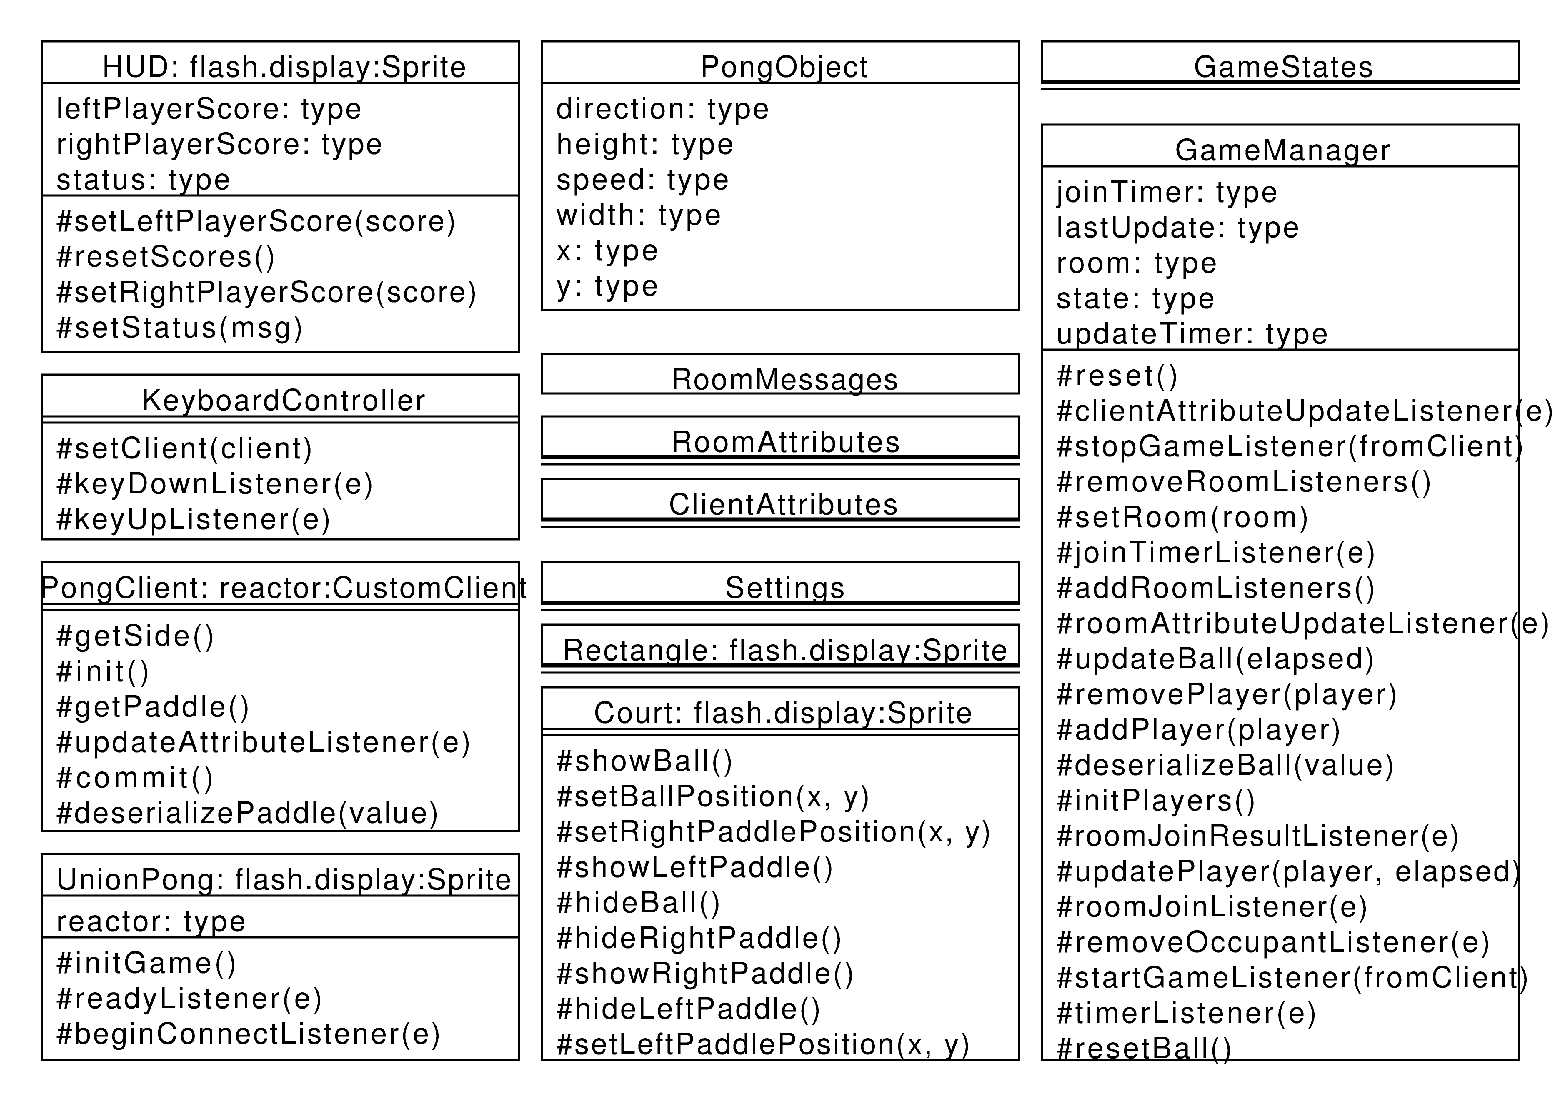
\includegraphics[scale=0.330000]{pics/UnionPong-manuallayout_fontembed.pdf}
\caption{The 13 classes in UnionPong client side ActionScript.}
\end{figure}

\section{Discussion}

\subsection{Interpretation and Validity of Object-Point Values}

The fact that UnionPong obtains much higher OP values indicating a
more complex API does not mean that the Union platform would be
somehow inferior. Instead, it highlights the nature of game
development at a different abstraction level. As we discussed in
Section IV.B, the platforms achieve the basic functionality of the
Pong game, such as synchronizing object movements and ball collisions
and bounces, in different ways: UnionPong uses game specific messages,
whereas TundraPong relies on the built-in functionality of the Tundra
platform. Otherwise, the two APIs are very similar regarding
networking. Both have an abstract container for the state, a Room in
Union, and a Scene in Tundra. An application can store own custom
state information as special attributes in the container, and the
system takes care of automatically synchronizing changes to the state
information. Both use callbacks heavily, for example to listen to new
clients entering the service (an event of Room in Union’s Reaktor and
in the RoomModule on the Union server separately, an event of the
Server core API object in Tundra server) and to attribute changes
received from the network. They both also allow sending simple ad-hoc
custom messages: Tundra uses them for game events such as informing of
a victory with the associated data; UnionPong uses them for
networking, including also paddle and ball movements, which Tundra
does automatically. These similarities indicate that the OP analysis
effectively captures the aforementioned differences in the scope and
the abstraction level of the platforms.

Looking at the OP data and considering the OP method, our
interpretation is that it succeeds in illustrating the difference in
scope and abstraction level between the two codebases. We have to ask
whether the OP method does that better than some other, perhaps
simpler, metrics would do. From previous research we know that the OP
method does succeed in identifying complexity that a simple LoC metric
would miss \cite{api-complexity-analysis}. Our data seems to support that same
conclusion, as the LoC measure would give even larger complexity
difference between the two implementations (115:565 for full
clients). Based on qualitative analysis, we think that the smaller
relative difference indicated by the OP data is more appropriate. Even
though UnionPong client needs to do more, and especially has many more
classes, most of the classes are very simple and most of the source
code is not very complex. Considering only static class information,
the difference would be even greater (27:180). TundraPong has
relatively long methods and a lot of function calls, which lead to
relative high MP count in the dynamic analysis (63:196). We think that
changes the final OP score to a realistic ratio (90:376). Based on the
OP data we cannot really say whether the tool and the OP method miss
something essential in the API complexity analysis. For example, the
OP method does not take into account anything specific to networking:
the need to think of connections, defining and sending network messages
etc. They are of course accounted for as normal data definitions and
function calls, but would some networking specific metric, for example
for the number of messages, be more useful instead? Arguably, they
present an additional complexity that the game developer has to
manage.

\subsection{Built-in Platform Logic vs. Custom Application Logic}

As TundraPong shows, implementing a game on an rich platform such as
Tundra can require a comparatively small amount of work. However,
custom game specific solutions for game object data, network messages,
movement inter/extrapolation and collisions can easily be more
powerful and even required. For example, if the game takes place on a
small spherical world, a mini planet, Tundra’s built-in Euclidean
movement techniques become suddenly much less useful. Therefore, the
logic underlying the Union platform and other similar smaller
libraries is sound. Game developers often need custom solutions, so
the platform just provides the lower level tools for messaging and
stays out of the way for the rest. However, optimizing and perfecting
for example movement synchronization is not trivial, thus it is often
useful to have a mature shared implementation for common operations.

\subsection{Complexity Metrics in Estimating Ease of Development}

Hatton criticized that software complexity metrics, including
cyclomatic complexity, have poor correlation with actual reported
defects in large software projects \cite{hatton}. He argued that none
of the various complexity metrics gives any better prediction than the
simplest metric of lines of code. In our study, however, the objective
is not to predict defects but to estimate development effort and ease
of development using particular APIs.

The recent metrics for the cognitive complexity of software may thus
be suitable, for example the Cognitive Information Complexity Measure
(CICM) reportedly satisfies all the criteria set for an effective
software complexity measure \cite{cicm}. It draws from research in
cognitive informatics and is based on calculating basic control
structures (BCS) from the code and assigning cognitive weights for
those constructs. The studies on cognitive complexity focus on
comprehensibility of the software when the source code is read. We
assume that it correlates with the ease of developing that piece of
code as well. However, we have been unable to find any automated tools
to calculate CICM or other BCS based metrics. Also, their objective is
to analyze complexity within individual functions, similarly to
cyclomatic complexity, whereas in API evaluation the overall program
structure may be more relevant.

\subsection{Limitations and Future Work}

The Pong game used as the minimal reference of a networked multiplayer
game in this study is very simplistic. Much of the complexity of real
networked games, and especially large scale commercial MMOGs, lies in
areas not addressed by this study: service reliability, availability,
restorability and scalability [1]. Networked programming in general is
also typically complex due to the need to handle several kinds of
error situations, such as lost data, dropped connections and conflicts
from simultaneous actions. The Pong reference implementations of this
study may well be limited in that they do not handle such issues in
the way a production quality game must handle, which probably
increases the complexities. However, both Pong games are built on very
high-level networked game platforms, which strive to hide the
complexity of networking from the developer. Whether and how they
really achieve that cannot be determined from the data of this study,
but would require a different analysis.

In future work the shortcoming of relying on too simple reference
games in API complexity analysis could be addressed in two
ways. First, we could analyze codebases of real production
games. However, typically a particular game exists only as a single
implementation, which prevents comparative analysis. Nevertheless, the
analysis could still provide valuable insight into assessing the
evolution of the complexity of the game, and the correlation of the
complexity with the monetary expenses of the development
effort. Second, we could develop a more complex reference game and
ensure its completeness. Such a reference game should be carefully
specified to cover all relevant areas of networked gaming, but still
remain small enough to allow implementation within a realistic
timeframe. Existing canonical implementations may provide a starting
point, as for example several commercial networked 3D first-person
shooter (FPS) games have been open sourced (Quake, Cube2), and at
least one high-level platform already features a FPS as a tutorial
(Torque3D).

We propose a collaborative effort, similar to the TodoMVC.com for web
platform comparisons \cite{todomvc}, to work on reference games for
API evaluation purposes. We suggest using \emph{refgames.org} for the purpose
and provide these example Pong's and our OP tool there as seed material.

\section{Conclusions}

Our study shows that software complexity metrics can be useful aids in
comparing APIs but so that human judgment is exercised in assessing
the plain numerical complexity values. The different metrics give
useful information on the overall characteristics of code bases and
can also highlight potential complexity hotspots for further study. 
A collaboratively composed collection of reference games on various platforms
seems like a fruitful way to get rich API comparisons in the future.

\section*{Acknowledgments}
The authors would like to thank Jonne Nauha from Adminotech for implementing most of TundraPong and providing the source for research purposes.
We also thank creators of the Union platform for providing their Pong example online, and for the nice and interestingly different platform overall.
We are greatful for the anonymous reviewers for insightful and helpful comments.
This work was supported by the NIMO (Nordic Interaction and Mobility Research Platform) project funded by the EU Interreg IVA North program, and by the Tekes Chiru project.

\bibliographystyle{IEEE}
\bibliography{IEEEabrv,bib}

\end{document}
